"..."
\chapter{xen}
VMM nato come opensoruce paravirtualizzato.
\begin{figure}[H]
	\caption{Architettura xen}
	\centering
	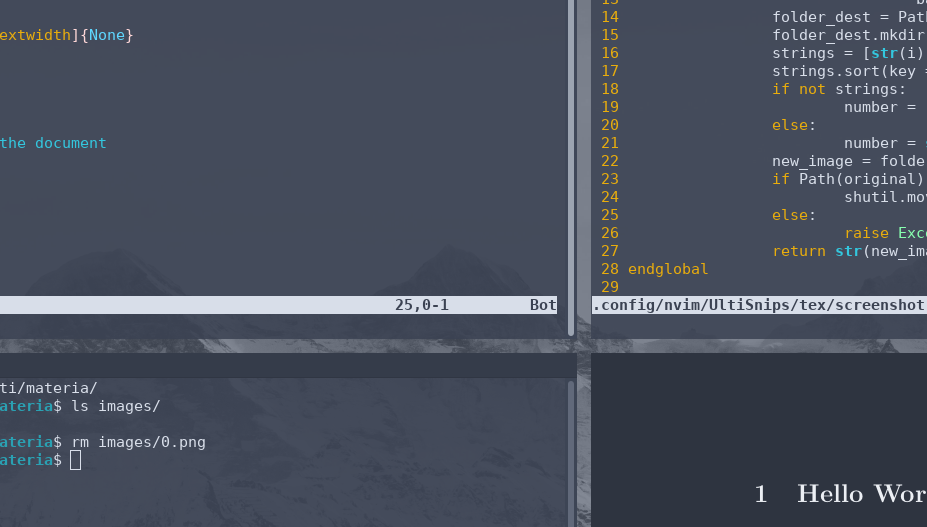
\includegraphics[width=0.8\textwidth]{/home/riccardoob/appunti/sistemi_operativi/images/0.png}
\end{figure}
Xen è un VMM di sistema, ovvero si appoggia direttamente sull'hardware e quindi può eseguire direttamente chiamate system call che necessita del rin 0.

Il vmm si occupa della virtualizzazione della CPU, della memoria e dei dispositivi per ogni macchina virtuale, qui definiti domain.

Xen offre una interfaccia di controllo in grado di gestire la divisione delle risorse tra i vari domini.
L'accesso a questa interfaccia è consentito soltanto da una speciale VM, la domain 0.

\section{Caratteristiche}
Data la natura \textbf{paravirtualizzata} delle VM gestite da xen, le VM possono eseguire direttamente system calls che vengono delegate al VMM tramite hypercalls.

Per quanto riguarda la \textbf{protezione}, i guest OS sono collocati nel ring 1.

\begin{figure}[H]
	\caption{Protezione e hypercalls guest OS}
	\centering
	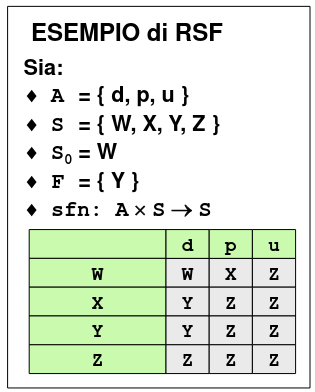
\includegraphics[width=0.85\textwidth]{/home/riccardoob/appunti/sistemi_operativi/images/1.png}
\end{figure}

\section{Gestione memoria e paginazione}

\subsubsection{Gestione della memoria}
Gli OS guest gestioscono la memoria virtuale mediante i meccanismi e le politiche tradizionali.

La soluzione adottata si basa sulle tabelle delle pagine delle VM:\\
Vengono mappate nella memoria fisica dal VMM (\textbf{shadow page tables}, possono essere accedute in scrittura soltanto dal VMM stesso ma sono disponibili in modalità read-only ai guest.

In caso di necessità di update, il VMM valuta la richiesta e la esegue.

Per alleggerire l'onere del procedimento di update, viene implementato il \textbf{memory split}, per permettere una maggiore efficienza delle hypercalls: xen risiede nei primi 64MB del virtual address space.

\begin{figure}[H]
	\caption{Struttura virtual address space- memory split}
	\centering
	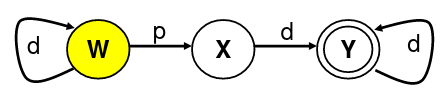
\includegraphics[width=0.6\textwidth]{/home/riccardoob/appunti/sistemi_operativi/images/2.png}
\end{figure}

I guest OS si occupano della paginazione, delegando al VMM la scrittura delle page table entries, una volta create sono disponibili in read-only per il guest che le ha richieste.

\begin{figure}[H]
	\caption{Creazione pagine dal VMM}
	\centering
	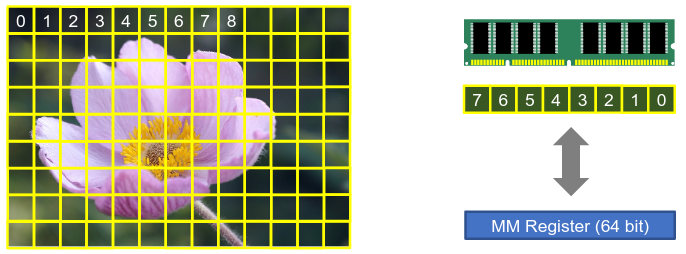
\includegraphics[width=0.7\textwidth]{/home/riccardoob/appunti/sistemi_operativi/images/3.png}
\end{figure}

\subsubsection{Creazione di un processo}

Il SO richiede una nuova tabella delle pagine al VMM:\\
\begin{itemize}
	\item aggiunte alla tabella le pagine appartenenti al segmento di xen
	\item xen registra la nuova tabella e acquisisce il diritto di scrittura esclusiva
	\item ogni successiva update da parte del guest provoca un protection-fault, comporta la verifica e l'aggiornamento della PT
\end{itemize}

\begin{figure}[H]
	\caption{Creazione di un processo}
	\centering
	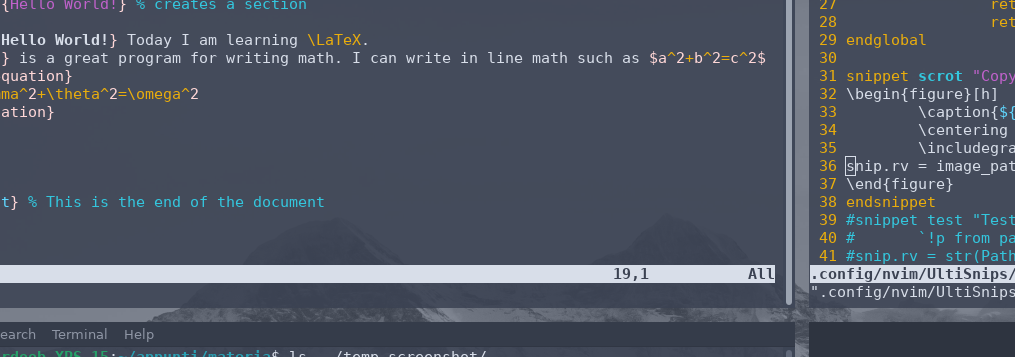
\includegraphics[width=0.85\textwidth]{/home/riccardoob/appunti/sistemi_operativi/images/4.png}
\end{figure}

\subsubsection{Balloon process}
Dato che la paginazione è a carico dei guest, il VMM necessita di avere un meccanismo per reclamare da altre macchine virtuali pagine di memoria meno utilizzate.
Su ogni macchina virtuale è in esecuzione un \textbf{ballon process} che, in caso di necessità, si "gonfia" per ottenere altre pagine che poi cede al VMM.

\section{Virtualizzazione della CPU}
Il VMM definisce una archiettura simile a quella del processore, con istruzioni privilegiate sostituite da opportune hypercalls.

Il VMM si occupa dello scheduling delle macchine virtuali: \textbf{Borrowed Virtual Time} scheduling algorithm:
\begin{itemize}
	\item si basa sulla nozione di virtual-time
	\item algoritmo general-purpose, consente di ottenre schedulazioni efficienti in caso di vincoli stringenti
\end{itemize}

Esistono due clock:
\begin{itemize}
	\item real-time, inizia al boot
	\item virtual-time, associato a VM, avanza solo quando la VM esegue
\end{itemize}

\begin{figure}[H]
	\caption{Virtualizzazione dell'I/O}
	\centering
	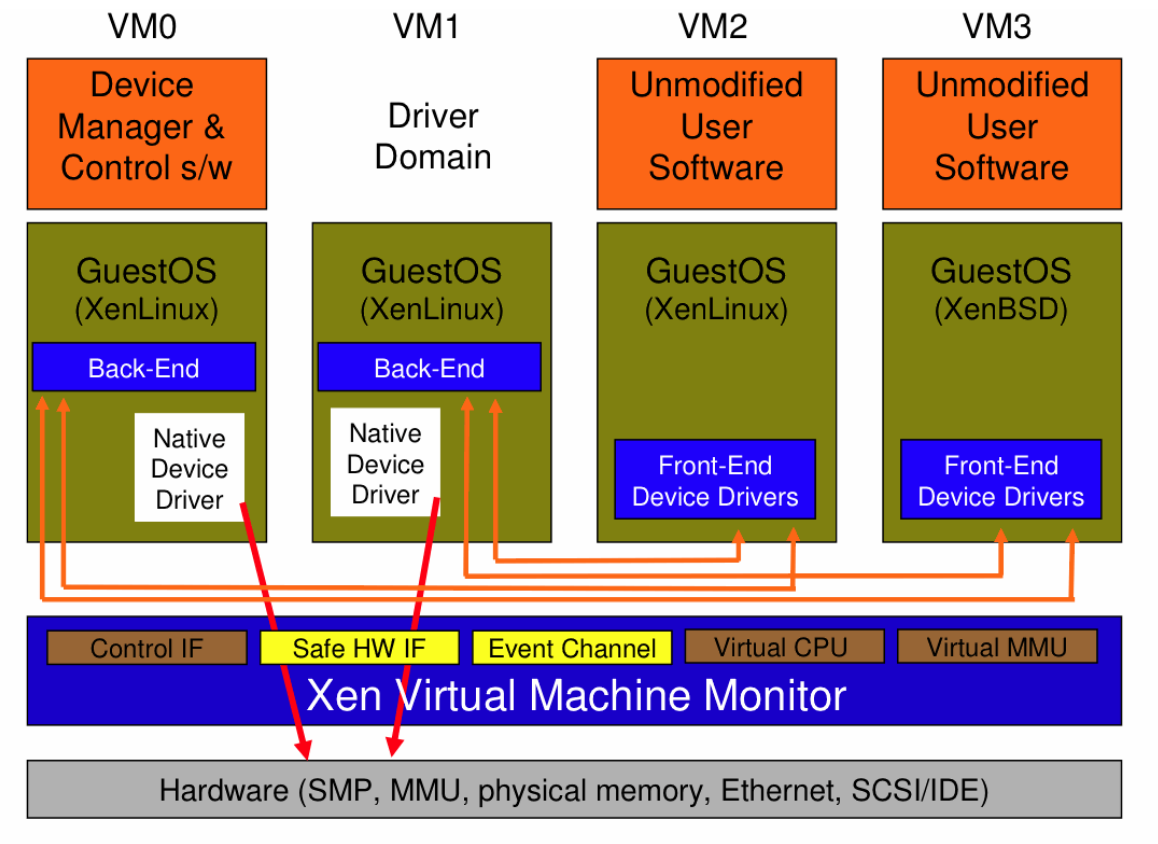
\includegraphics[width=0.7\textwidth]{/home/riccardoob/appunti/sistemi_operativi/images/5.png}
\end{figure}

Esiste un \textbf{back-end driver} per ogni dispositivo, il suo driver è isolato all'interno di una particolare macchine virtuale (tipicamente dom0), ha accesso diretto all'hardware.

Ogni guest prevede un \textbf{front-end driver} virtuale semplificato che consente l'accesso al device tramite il back-end.

Questa tecnica comporta una semplificazione della portabilità a scapito della necessità di comunicaazione don il back-end attraverso degli asynchronous I/O rings.
\begin{figure}[H]
	\caption{I/O rings}
	\centering
	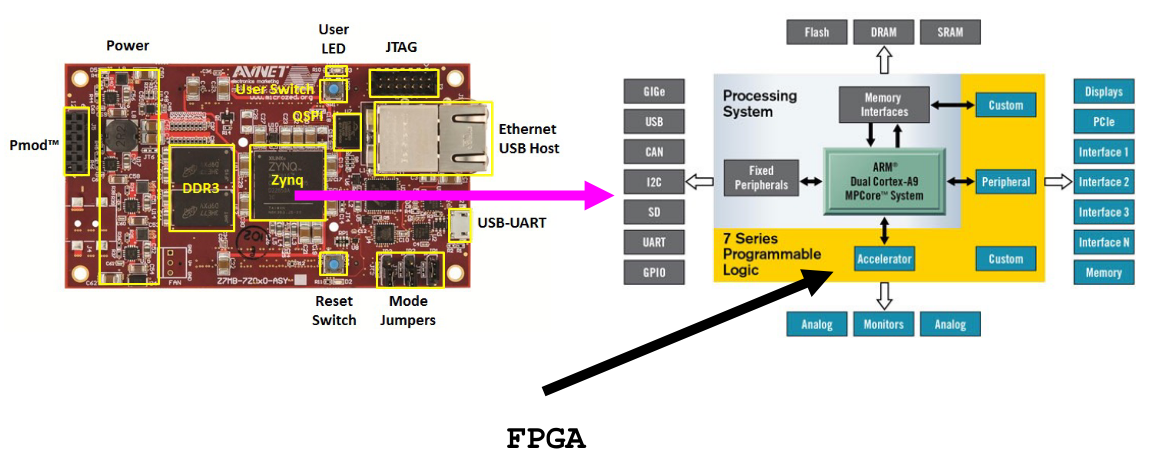
\includegraphics[width=0.75\textwidth]{/home/riccardoob/appunti/sistemi_operativi/images/6.png}
\end{figure}

\section{Gestione interruzioni e eccezioni}
La gestione delle interruzione viene virtualizzata in modo da lasciare a ogni guest la gestione delle interruzioni, il vettore punta direttamente alle routine del kernel guest.

Il page-fault è un caso particolare, nel quale è necessario l'intervento del VMM, in quanto l'indirizzo che ha provocato il page-fault è contenuto nel registro CR2, inaccessibile al guest: il guest punta a codice xen che esegue una copia del CR2 all'interno di una variabile nello spazio guest.

\section{Live migration in xen}
La migrazione è \textbf{guest-based}: il comando di migrazione viene eseguite da un demone di migrazione nel domain0 del server di origine della macchine da migrare.

La realizzazione si basa sulla modalità pre-copy, le pagine da migrare vengono compresse per ridurre l'occupazione di banda.

\begin{figure}[H]
	\caption{Migrazione live}
	\centering
	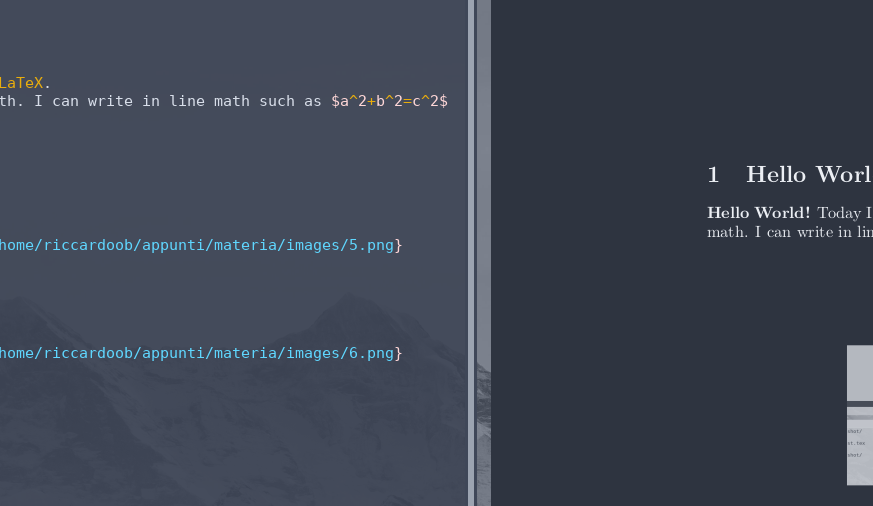
\includegraphics[width=0.8\textwidth]{/home/riccardoob/appunti/sistemi_operativi/images/7.png}
\end{figure}

